\documentclass[16pt,aspectratio=169]{beamer}

\usetheme{metropolis}

\definecolor{mDarkBrown}{HTML}{FF5722}
\definecolor{mDarkTeal}{HTML}{263238}
\definecolor{mLightBrown}{HTML}{FF5722}

\usepackage{booktabs}
\usepackage{graphicx}
\usepackage{hyphenat}

\usepackage{polyglossia}
\setdefaultlanguage[variant=british]{english}
\usepackage[english=british]{csquotes}

\defaultfontfeatures{Ligatures=TeX}
\setmainfont{Source Sans Pro}
\setsansfont[Scale=MatchLowercase]{Source Sans Pro}
\setmonofont[Scale=MatchLowercase]{Source Code Pro}

\renewcommand{\vec}[1]{\ensuremath{\mathbf{#1}}}
\newcommand{\mat}[1]{\ensuremath{\vec{#1}}}
\newcommand{\tr}{\ensuremath{\intercal}}
\newcommand{\R}{\ensuremath{\mathbb{R}}}

\definecolor{red500}{HTML}{F44336}

\title{New uses for old tools}
\subtitle{An introduction to mathematical programming}
\author{Dr Gianluca Campanella}
\date{29\textsuperscript{th} April 2017}

\begin{document}

\maketitle

\begin{frame}{Contents}
    \tableofcontents
\end{frame}

\section{Mathematical programming}

\begin{frame}{What is mathematical programming?}
    \only<1>{%
        \begin{itemize}
            \item Also known as (mathematical) \emph{optimisation}
            \item Goal is to select the `best' element from some set of
                  available alternatives
        \end{itemize}
        \vfill
        Typically we have an \emph{objective} function, e.g.\
        $f\,:\,\R^{p} \to \R$, that:
        \begin{itemize}
            \item Takes $p$ inputs as a vector, e.g.\ $\vec{x} \in \R^{p}$
            \item Maps the input to some output value $f(\vec{x}) \in \R$
        \end{itemize}
        We want to find the \emph{optimal} $\vec{x}^{\star}$ that minimises (or
        maximises) $f$}
    \only<2>{%
        \begin{itemize}
            \item Many ML methods rely on minimisation of \emph{cost functions}
        \end{itemize}
        \vfill
        \begin{columns}
            \begin{column}{0.35\textwidth}
                \begin{block}{\centering Linear regression}
                    \centering
                    \[
                        \operatorname{MSE}(\hat{\vec{\beta}}) = \frac{1}{n} \sum_{i} \left( \hat{y}_{i} - y_{i} \right)^{2}
                    \]
                    where $\hat{y}_{i} = \vec{x}_{i}^{\tr} \hat{\vec{\beta}}$
                \end{block}
            \end{column}
            \begin{column}{0.65\textwidth}
                \begin{block}{\centering Logistic regression}
                    \centering
                    \[
                        \operatorname{LogLoss}(\hat{\vec{\beta}}) = - \sum_{i} \left[ y_{i} \log \hat{p}_{i} + (1 - y_{i}) \log (1 - \hat{p}_{i}) \right]
                    \]
                    where $\hat{p}_{i} = \operatorname{logit}^{-1}(\vec{x}_{i}^{\tr} \hat{\vec{\beta}})$
                \end{block}
            \end{column}
        \end{columns}}
\end{frame}

\begin{frame}{Local and global optima}
    \begin{columns}
        \begin{column}{0.5\textwidth}
            \centering
            A function may have \emph{multiple} optima \\[1em]
            $\downarrow$ \\[1em]
            Some will be \emph{local}, some will be \emph{global} \\[2em]
        \end{column}
        \begin{column}{0.5\textwidth}
            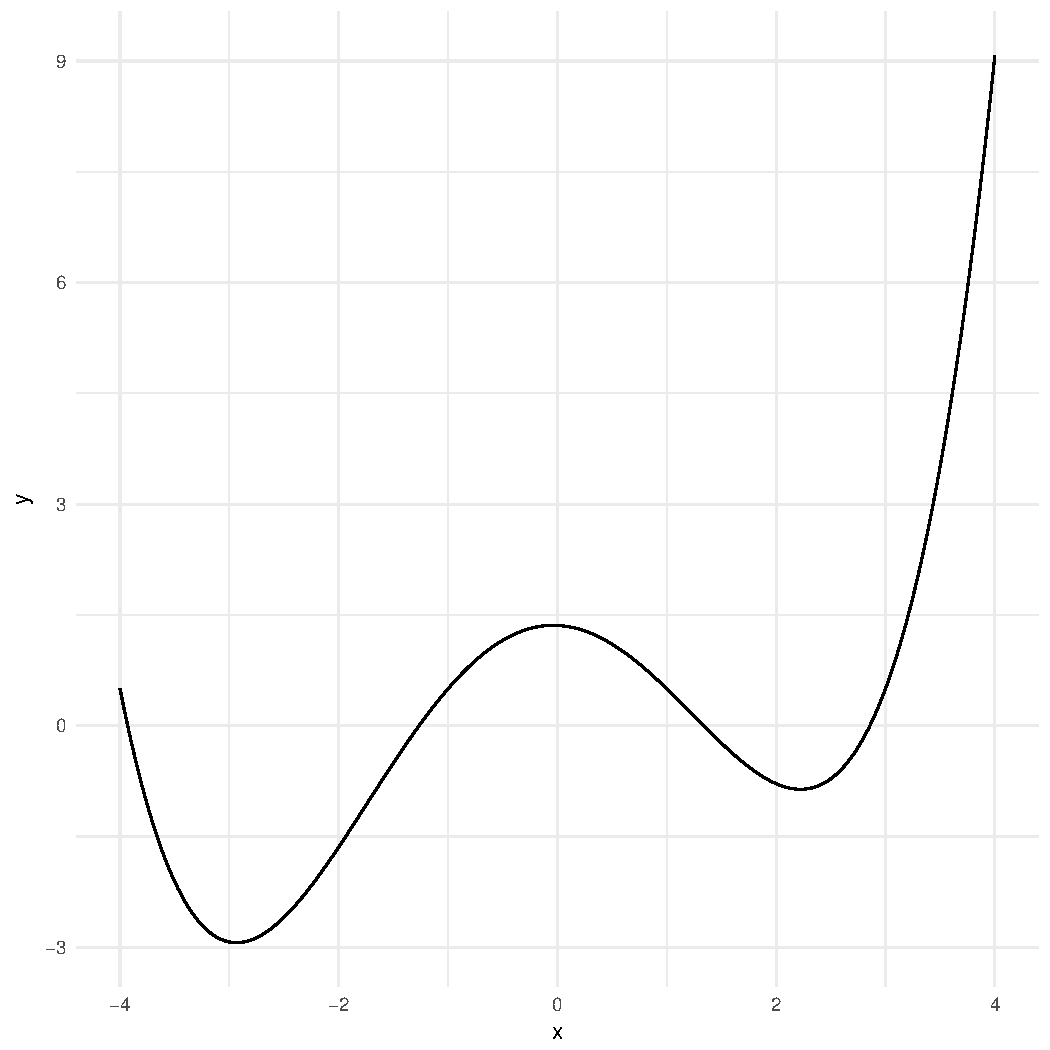
\includegraphics[height=0.95\textheight]{figures/local_vs_global_minima}
        \end{column}
    \end{columns}
\end{frame}

\begin{frame}{Hard optimisation problems}
    Consider these three functions:
    \begin{align*}
        f\,&:\,\R^{100} \to \R \\
        g\,&:\,[0, 1]^{100} \to \R \\
        h\,&:\,\{0, 1\}^{100} \to \R
    \end{align*}
    \vfill
    Which one is `harder' to optimise, and why?
\end{frame}

\begin{frame}{Combinatorial optimisation}
    Combinatorial problems like optimising $h\,:\,\{0, 1\}^{100} \to \R$ are
    intrinsically hard
    \begin{itemize}
        \item Need to try all $2^{100} \approx 1.27 \times 10^{30}$ combinations
        \item \emph{Variable selection} is a notable example
    \end{itemize}
    \vfill
    \begin{block}{Side note}
        If $h$ is continuous and we're actually constraining
        $\vec{x} \in \{0, 1\}^{100}$, approximate solutions (\emph{relaxations})
        are normally easier to obtain
    \end{block}
\end{frame}

\begin{frame}{Numerical optimisation using directional information}
    \begin{columns}
        \begin{column}{0.5\textwidth}
            \centering
            Function is differentiable \\ (analytically or numerically) \\[1em]
            $\downarrow$ \\[1em]
            \textbf{Gradient gives a search \emph{direction}} \\
            and \\
            Hessian can be used to confirm optimality
        \end{column}
        \begin{column}{0.5\textwidth}
            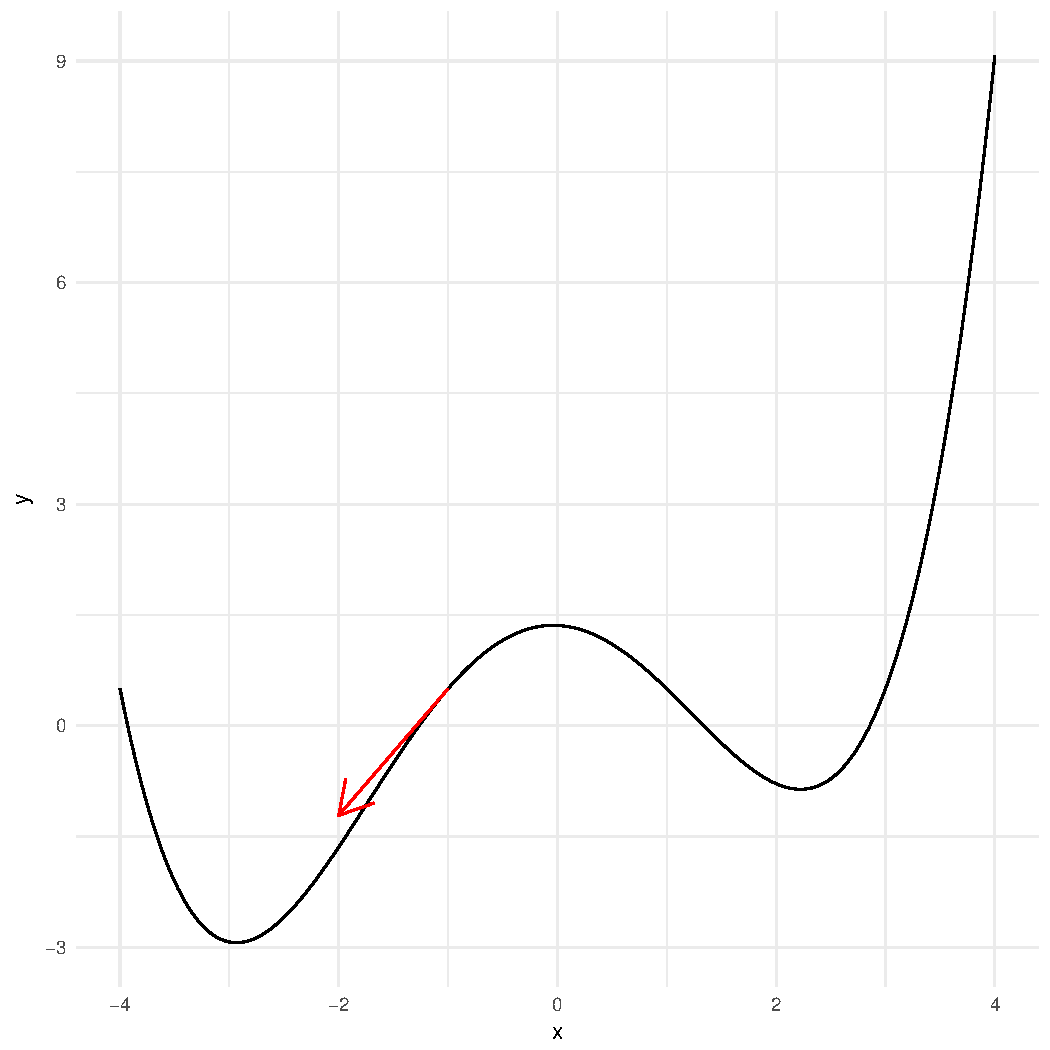
\includegraphics[height=0.95\textheight]{figures/derivative}
        \end{column}
    \end{columns}
\end{frame}

\begin{frame}{Convex functions}
    \begin{columns}
        \begin{column}{0.5\textwidth}
            \centering
            \textbf{Function is \emph{convex}} \\[1em]
            $\downarrow$ \\[1em]
            Any local minimum is \\ also a global minimum
        \end{column}
        \begin{column}{0.5\textwidth}
            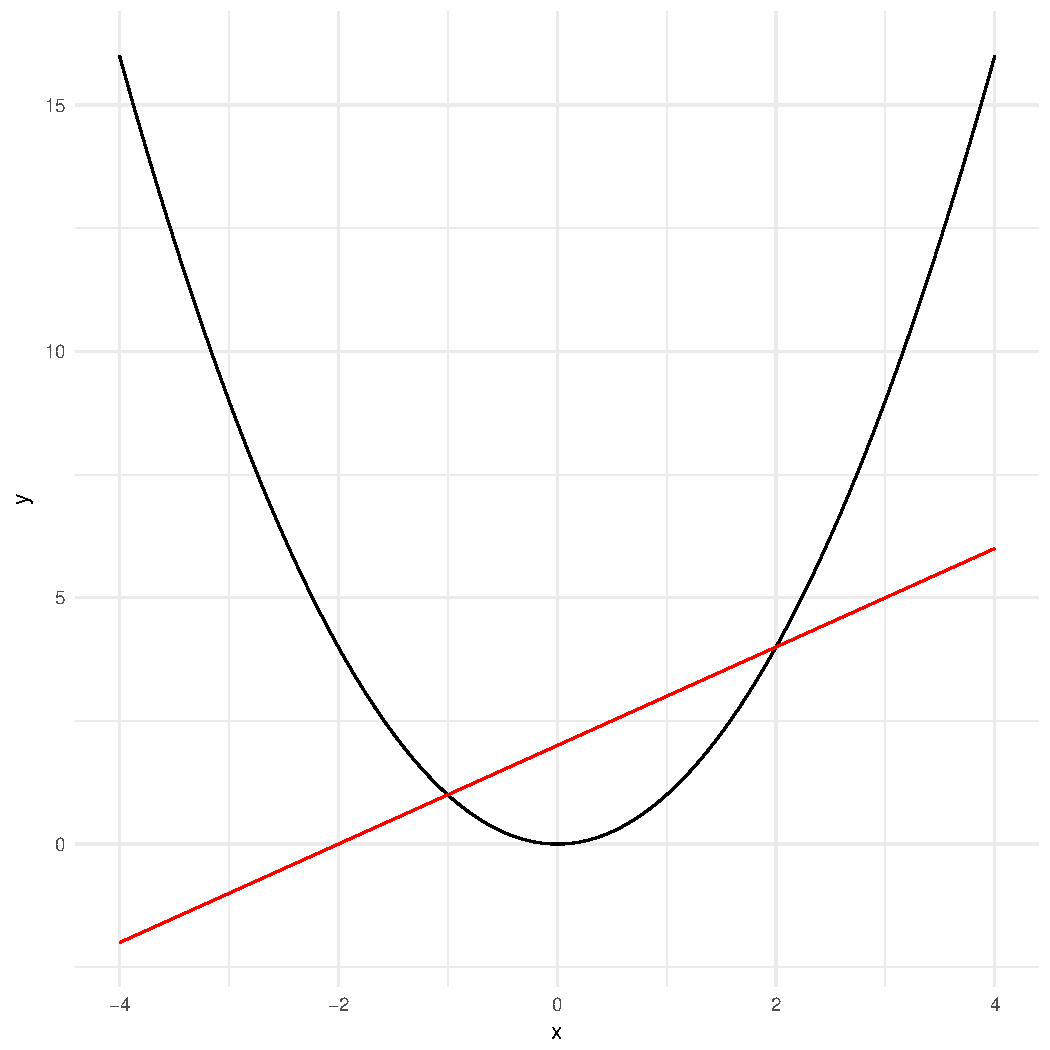
\includegraphics[height=0.95\textheight]{figures/convex_function}
        \end{column}
    \end{columns}
\end{frame}

\begin{frame}{Constrained optimisation}
    What about $g\,:\,[0, 1]^{100} \to \R$?
    \begin{itemize}
        \item Harder than $f\,:\,\R^{100} \to \R$\ldots~but not much
        \item Directional information still useful
        \item Need to ensure search strategy doesn't escape the
              \emph{feasible region}
    \end{itemize}
\end{frame}

\section{Linear and quadratic programs}

\begin{frame}{Linear programs}
    \only<1>{%
        \begin{align*}
            \max_{\vec{x}} \ &\ \vec{c}^{\tr} \vec{x} \\
            \text{s.t.}    \ &\ \mat{A} \vec{x} \leq \vec{b} \\
                           \ &\ \vec{x} \geq \vec{0}
        \end{align*}
        \begin{itemize}
            \item Linear objective, linear constraints
            \item Linear objective is convex $\leadsto$ global maximum
            \item An optimal solution need not exist:
                  \begin{itemize}
                      \item Inconsistent constraints $\leadsto$ infeasible
                      \item Feasible region unbounded in the direction of
                            the gradient of the objective
                  \end{itemize}
        \end{itemize}}
    \only<2>{%
        \begin{columns}
            \begin{column}{0.5\textwidth}
                \begin{align*}
                    \max_{x,\,y} \ &\ 3x + 4y \\
                    \text{s.t.} \ &\ x + 2y \leq 14 \\
                                \ &\ 3x - y \geq 0 \\
                                \ &\ x - y \leq 2
                \end{align*}
            \end{column}
            \begin{column}{0.5\textwidth}
                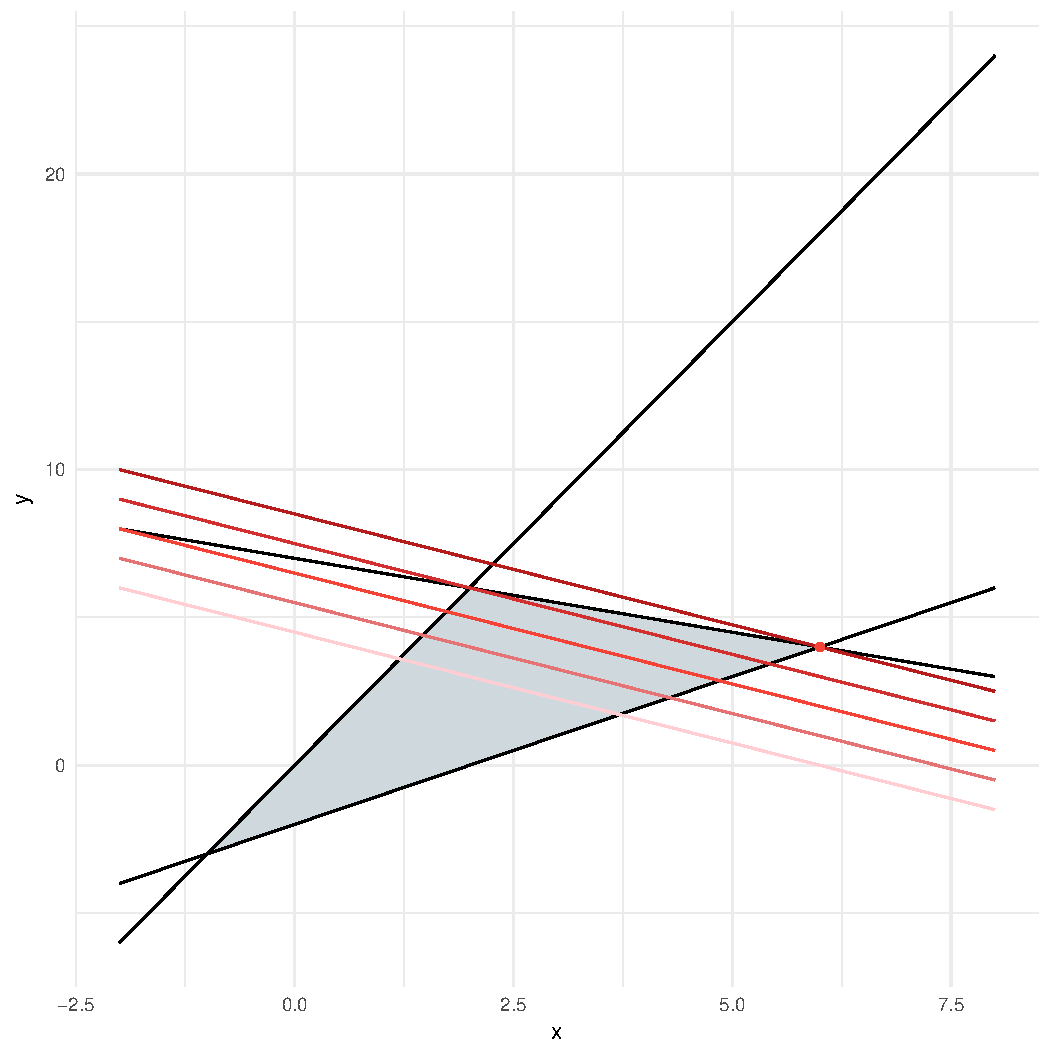
\includegraphics[height=0.95\textheight]{figures/lp}
            \end{column}
        \end{columns}}
    \only<3>{%
        Linear programs can be solved efficiently using:
        \begin{itemize}
            \item Simplex algorithm
            \item Interior\hyp{}point (barrier) methods
        \end{itemize}
        Performance is \emph{generally} similar, but might differ drastically
        for specific problems}
\end{frame}

\begin{frame}{Convex quadratic programs}
    \only<1>{%
        \begin{align*}
            \min_{\vec{x}} \ &\ \frac{1}{2} \vec{x}^{\tr} \mat{Q} \vec{x} + \vec{c}^{\tr} \vec{x} \\
            \text{s.t.}    \ &\ \mat{A} \vec{x} \preceq \vec{b} \\
                           \ &\ \vec{x} \succeq \vec{0}
        \end{align*}
        \begin{itemize}
            \item Quadratic objective, quadratic constraints
            \item Are quadratic objectives always convex?
            \item $\mat{Q}$ must be (semi)definite
        \end{itemize}}
    \only<2>{%
        Quadratic programs can be solved efficiently using:
        \begin{itemize}
            \item Active set method
            \item Augmented Lagrangian method
            \item Conjugate gradient method
            \item Interior\hyp{}point (barrier) methods
        \end{itemize}}
\end{frame}

\begin{frame}{LPs and QPs in Python}
    Many Python libraries exist:
    \vfill
    \begin{block}{Linear programming}
        \begin{itemize}
            \item PuLP
            \item Google Optimization Tools
            \item \texttt{clpy}
        \end{itemize}
    \end{block}
    \begin{block}{Convex quadratic programming}
        \begin{itemize}
            \item CVXOPT
            \item CVXPY
        \end{itemize}
    \end{block}
\end{frame}

\section{Regression problems as LPs and QPs}

\begin{frame}{Linear regression}
    We can rewrite the least\hyp{}squares problem
    \[
        \min_{\vec{x}} \ \left|\left|\,\mat{A}\vec{x} - \vec{b}\,\right|\right|_{2}^{2}
        = \sum_{i} \varepsilon_{i}^{2}
    \]
    as the convex quadratic objective
    \[
        f(\vec{x}) = \vec{x}^{\tr} \mat{A}^{\tr} \mat{A} \vec{x} - 2 \vec{b}^{\tr} \mat{A} \vec{x} + \vec{b}^{\tr} \vec{b}
    \]
    \vfill
    \begin{block}{Side note}
        Setting the gradient to 0 and solving for $\vec{x}$ recovers the normal
        equations:
        \[
            \nabla f = 2 \mat{A}^{\tr} \mat{A} \vec{x} - 2 \mat{A}^{\tr} \vec{b} = 0
            \quad\leadsto\quad
            \mat{A}^{\tr} \mat{A} \vec{x} = \mat{A}^{\tr} \vec{b}
            \quad\leadsto\quad
            \vec{x}^{\star} = \left( \mat{A}^{\tr} \mat{A} \right)^{-1} \mat{A}^{\tr} \vec{b}
        \]
    \end{block}
\end{frame}

\begin{frame}{Regularised linear regression}
    Let's add a penalisation term:
    \[
        \min_{\vec{x}} \ \left|\left|\,\mat{A}\vec{x} - \vec{b}\,\right|\right|_{2}^{2}
        + \textcolor{red500}{\lambda \left|\left|\, \vec{x} \,\right|\right|_{2}^{2}}
    \]
    Our quadratic objective becomes:
    \[
        f(\vec{x}) = \vec{x}^{\tr} \left( \mat{A}^{\tr} \mat{A} + \textcolor{red500}{\lambda \mat{I}_{p}} \right) \vec{x} - 2 \vec{b}^{\tr} \mat{A} \vec{x} + \vec{b}^{\tr} \vec{b}
    \]
    \vfill
    \begin{block}{Side note}
        This is a good trick to use when the columns of $\mat{A}$ are not
        perfectly independent
    \end{block}
\end{frame}

\begin{frame}{Constraints on $\vec{x}$}
    \begin{block}{Nonnegativity}
        \begin{itemize}
            \item $\vec{x} \geq \vec{0}$
            \item Parameters known to be nonnegative, e.g.\ intensities or rates
        \end{itemize}
    \end{block}
    \begin{block}{Bounds}
        \begin{itemize}
            \item $\vec{l} \leq \vec{x} \leq \vec{u}$
            \item Prior knowledge of permissible values
        \end{itemize}
    \end{block}
    \begin{block}{Unit sum}
        \begin{itemize}
            \item $\vec{x} \geq \vec{0}$ and $\vec{1}^{\tr}_{p} \vec{x} = \vec{1}$
            \item Useful for proportions and probability distributions
        \end{itemize}
    \end{block}
\end{frame}

\begin{frame}{Least squares \textit{vs} least absolute deviations}
    \only<1>{%
        \begin{center}
            \large%
            Why do we minimise \emph{squared} residuals?
        \end{center}
        \begin{itemize}
            \item Stable, unique, analytical solution
            \item Not very robust!
        \end{itemize}}
    \only<2>{%
        \begin{block}{Least \emph{absolute} deviations}
            \begin{itemize}
                \item Predates least squares by around 50 years (Bošković)
                \item Adopted by Laplace, but shadowed by Legendre and Gauss
                \item \emph{Robust}
                \item Possibly multiple solutions
            \end{itemize}
        \end{block}}
\end{frame}

\begin{frame}{Robust regression}
    We can rewrite the LAD problem
    \[
        \min_{\vec{x}} \ \left|\left|\,\mat{A}\vec{x} - \vec{b}\,\right|\right|_{1}
        = \sum_{i} \left| \varepsilon_{i} \right|
    \]
    as the linear program
    \begin{columns}
        \begin{column}{0.475\textwidth}
            \begin{align*}
                \min_{\vec{x}, \vec{t}} \ &\ \vec{1}_{n}^{\tr} \vec{t} \\
                \text{s.t.}             \ &\ -\vec{t} \leq \mat{A} \vec{x} - \vec{b} \leq \vec{t} \\
                                          &\ \vec{t} \in \R^{n}
            \end{align*}
        \end{column}
        \begin{column}{0.05\textwidth}
            \centering%
            or
        \end{column}
        \begin{column}{0.475\textwidth}
            \begin{align*}
                \min_{\vec{x}, \vec{u}, \vec{v}} \ &\ \vec{1}_{n}^{\tr} \vec{u} + \vec{1}_{n}^{\tr} \vec{v} \\
                \text{s.t.}                      \ &\ \mat{A} \vec{x} + \vec{u} - \vec{v} = \vec{b} \\
                                                   &\ \vec{u}, \vec{v} \geq \vec{0}
            \end{align*}
        \end{column}
    \end{columns}
\end{frame}

\begin{frame}{Quantile regression}
    \begin{columns}
        \begin{column}{0.5\textwidth}
            Let's now introduce a weight \textcolor{red500}{$\tau \in [0, 1]$}
            \begin{align*}
                \min_{\vec{x}, \vec{u}, \vec{v}} \ &\ \textcolor{red500}{\tau}\,\vec{1}_{n}^{\tr} \vec{u} + \textcolor{red500}{(1 - \tau)} \vec{1}_{n}^{\tr} \vec{v} \\
                \text{s.t.}                      \ &\ \mat{A} \vec{x} + \vec{u} - \vec{v} = \vec{b} \\
                                                   &\ \vec{u}, \vec{v} \geq \vec{0}
            \end{align*}
            This is the $\tau^{\text{th}}$ \textbf{quantile regression} problem
        \end{column}
        \begin{column}{0.5\textwidth}
            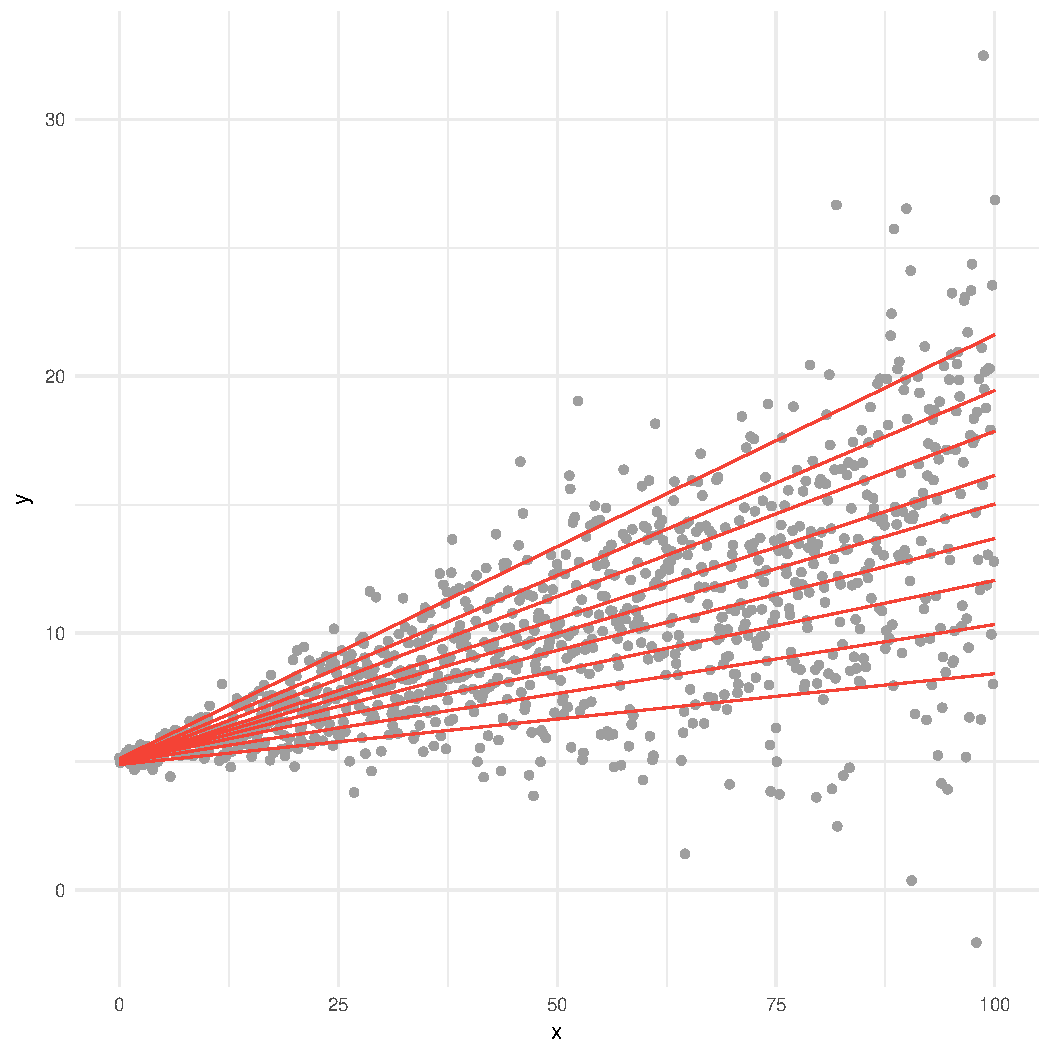
\includegraphics[height=0.95\textheight]{figures/quantile_regression}
        \end{column}
    \end{columns}
\end{frame}

\section{An application to portfolio theory}

\begin{frame}{Example}
    \begin{itemize}
        \item Consider these two assets:
              \begin{description}
                  \item[A] Equally likely to go up 20\% or down 10\% in a year
                  \item[A] Equally likely to go up 20\% or down 10\% in a year
              \end{description}
        \item Assume they're perfectly inversely correlated
        \item How would you allocate your money?
    \end{itemize}
    \pause
    \begin{center}
        \large%
        The portfolio 50\% \textbf{A} + 50\% \textbf{B} goes up 5\% every year!
    \end{center}
\end{frame}

\begin{frame}{Mean\hyp{}variance approach of Markowitz}
    \only<1>{%
        Given historical ROIs, denoted $r_{i}(t)$ for asset $i$ at time
        $t \leq T$, we can compute:
        \begin{itemize}
            \item The \emph{reward} of asset $i$:
                  \[
                      \text{reward}_{i} = \frac{1}{T} \sum_{t} r_{i}(t)
                  \]
            \item The \emph{risk} of asset $i$:
                  \[
                      \text{risk}_{\,i} = \frac{1}{T} \sum_{t} \left[ r_{i}(t) - \text{reward}_{i} \right]^{2}
                  \]
        \end{itemize}
        \vfill
        We can compute the same quantities for a \emph{portfolio}
        $\vec{x} \geq \vec{0}$, $\vec{1}^{\tr}_{p} \vec{x} = \vec{1}$}
    \only<2>{%
        Our objective is to \emph{maximise reward} and \emph{minimise risk}
        \vfill
        Instead, we solve
        \[
            \max_{\vec{x}} \ \text{reward}(\vec{x}) - \mu\,\text{risk}(\vec{x})
        \]
        for multiple values of the \emph{risk aversion parameter} $\mu \geq 0$
        \vfill
        \begin{itemize}
            \item Linear constraints: $\vec{x} \geq \vec{0}$,
                  $\vec{1}^{\tr}_{p} \vec{x} = \vec{1}$
            \item What about the objective function?
        \end{itemize}}
    \only<3>{%
        \begin{center}
            \large%
            Why is variance a reasonable measure of risk?
        \end{center}
        \vfill
        \begin{itemize}
            \item Variance\hyp{}based measures are not monotonic
            \item Quantile\hyp{}based measures (e.g.\ VaR) are not subadditive
            \item The loss beyond the VaR is ignored
        \end{itemize}}
\end{frame}

\begin{frame}{Other risk measures}
    Artzner et al.\ provided a foundation for `coherent' risk measures:
    \begin{itemize}
        \item Expected shortfall
        \item Conditional VaR (CVaR)
        \item $\alpha$\hyp{}risk
    \end{itemize}
    \vfill
    \pause
    \begin{block}{Linear programming solutions}
        \begin{itemize}
            \item Portfolios with CVaR constraints are linear programs
            \item $\alpha$\hyp{}risk models are $\alpha^{\text{th}}$ quantile
                  regression problems
        \end{itemize}
    \end{block}
\end{frame}

\begin{frame}{Recap}
    \begin{itemize}
        \item Optimisation is at the core of what we do!
        \item Some problems are much harder than others $\leadsto$ convexity
        \item LPs and QPs are `easy', with plenty of tools available
        \item Different commonly used regression models are actually LPs or QPs
        \item So are some portfolio allocation models!
    \end{itemize}
\end{frame}

\end{document}

